\addsection{Programming generic nodes}

\begin{figure}[htb]
  \centering 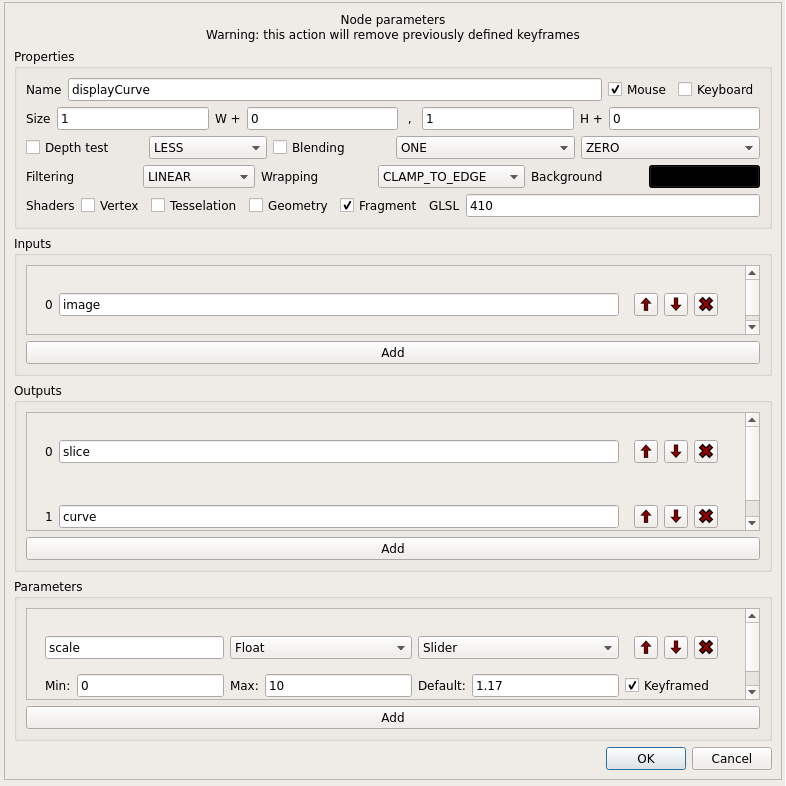
\includegraphics[width=\linewidth]{imgs/generic-settings.png} 
  \caption{\label{fig:generic-settings}Settings of a generic node.}
\end{figure}

\noindent Generic nodes provide users with the ability to precisely customize
processes to their needs by writing GLSL shaders directly from inside
the user interface. Most of the nodes available in Gratin are in fact
designed with generic nodes and their code might be directly modified
by users.  The creation of a generic node begins with the filling of a
dialog box where users specify important parameters of a GLSL shader
(Fig.~\ref{fig:generic-settings}):
\begin{itemize}
 \setlength\itemsep{0cm}
\item Properties: contains the name and other general parameters for
  the node. Check mouse and/or keyboard will grant access to mouse
  positions and keyboard keys in the shaders. The size of the output
  images are chosen via a function of the input texture sizes W and H
  (0 if no input). The user may also enable the depth test (with
  commonly used OpenGL functions), the blending, the filtering and the
  wrapping used for the output textures (see the OpenGL documentation
  - \url{https://www.opengl.org/} - for more information on how these
  options will affect the resulting images). Finally, the user can
  decide which shaders to activate
  (vertex/tesselation/geometry/fragment), choose the GLSL version and
  a default background color.
\item Inputs/outputs: choose the number of input
  (resp. output) images and modify their names. Chosen names will be
  directly used inside the shaders.
\item Parameters: add/remove necessary parameters. For each
  parameter, one may choose a name, a type (int/float/vec2/etc) and
  how it should appear in the node interface (slider/spin/etc). Min,
  max and default values should also be provided. Finally, checking
  the keyframed checkbox will allow the parameter to be controlled by
  keyframe curves.
\end{itemize}
%
Once the settings have been chosen, users may customize the node behavior
by writing GLSL code and observing results in real-time. Input and
output names are used to automatically generate the head of the
shaders. All the parameters are also available via generated uniform
variables. In the following, we present the different types of generic
nodes currently available in Gratin. For more information about how to
program using GLSL, visit:
\url{https://www.opengl.org/documentation/glsl/}. The provided
pipeline samples also illustrate how each of these generic node has
been used to produce different effects.

\remark{Remark: modifying the settings of a node will remove all previously defined keyframes for this node} 
% Romain: Je me rappelle plus pourquoi on avait mis ca et je comprend pas: and make also make shaders incorrect.}

\addsubsection{Generic image node} 
%
This node permits to analyze, manipulate and visualize input textures
(e.g., colored images, g-buffers).  As commonly done for image
processing in OpenGL, a simple quad is drawn in the viewport so that
input textures can be easily accessed and mapped to create outputs
containing specific effects.  This node may be used to create one-pass
custom complex shaders (as in
\href{https://www.shadertoy.com/}{Shadertoy} for instance), to mix
input images, to create various patterns and so on.
Implementation-wise, user-specified GLSL version, input and output
texture names are automatically used to generate the header of the
shader.  By default, the fragment shader simply makes a copy of the
first input texture.

\vspace{0.5cm}
\addsubsection{Generic buffers and grid nodes}
They let users apply
any effect to 3D meshes by customizing vertex, tessellation, geometry
and fragment shaders.  The main difference between object and grid
node types is that the former loads a mesh in OBJ format, while the
latter creates a planar grid.  In the case of the grid node,
tessellation is chosen by the user in the dedicated interface;
vertices are then typically displaced according to input GLSL code.
As with other generic nodes, any number of textures might be provided
as input (such as color or normal maps for instance).  Outputs are
typically in the form of g-buffers or renderings for further 3D or 2D
processing respectively.  A trackball camera is associated to this
node so that users may manipulate their object in the viewer panel.
In both cases, mesh positions, normals, tangents and texture
coordinates are directly sent as vertex attributes.  Consequently, the
header of the vertex shader is adapted to grant access to these
attributes.

\vspace{0.5cm}
\addsubsection{Generic splat node} 
This node permits to manipulate point
sprites and is useful to control particles, visualizations or even
image warpings.  The particularity here is to be able to modify splat
sizes and locations (possibly using overlapping and blending) to
obtain specific effects.  The interface permits to control the number
of rendered sprites, and their behavior is controlled through GLSL
code.  In practice, it works by sending a set of point sprites to the
GPU, with one splat per pixel by default.  Shader headers for the
generic splat node contain the position of the splat (as an attribute
in the vertex shader), as well as uniform variables.  The remainder of
the shader can be freely modified.

\vspace{0.5cm}
\addsubsection{Generic pyramid node} 
%
This node creates one or more mipmaped textures where one can control
how each level is computed.  It might be used for the creation of
usual mipmaps, but also for multiscale analysis (Gaussian or Laplacian
pyramids) or to compute global information such as the mean and
variance of an input image.  The shader header is automatically
generated and contains variables such as the number of levels and
flags to know whether the top or bottom of the pyramid have been
reached.  In addition, the previously computed level of each input
texture is automatically added to the GPU program as a uniform
sampler.  Users thus only have to describe per-level operations in a
specific order (top-down or bottom-up) in the GLSL code.  The
resulting pyramids are stored as mipmaps.  Further connected nodes may
thus easily access any texture level via GLSL built-in functions such
as \textit{textureLod()}.

\vspace{0.5cm}
\addsubsection{Generic ping-pong node} 
%
This node provides another useful feature commonly used in GPU
programming to implement iterative processes.  The same process is
applied at each internal pass, and repeated a number of times
specified by the user.  Such a type of node may be used to iteratively
accumulate or propagate some information in the output textures.  In
practice, it uses a pair of textures for internal multiple passes,
with one texture being read and the other written on even passes, and
the opposite on odd passes.  However, this is not apparent to the
user: we automatically generate a header that gives access to the
resulting texture of the previous internal pass, as well as the
current pass number.  Note that such a ping-pong architecture could
not be created manually by connecting simpler nodes, since our graph
is acyclic.

\remark{Remark: when opening a pipeline containing a ping-pong node, it will by default be initialized and run for the default number of passes. 
This might lead to important lags when each pass is a time-consuming process.} 

